\chapter{Programmazione dinamica}
\section{Motivazioni}
Si consideri il problema del cammino minimo di un grafo da $s$ a $t$.\\
\centerline{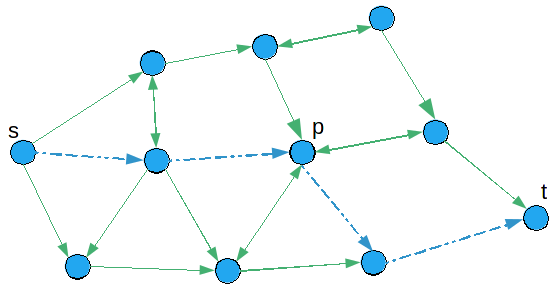
\includegraphics[height=4.25cm]{images/graph37.png}}
\subsection{Osservazione 1}
Se il cammino minimo $(s,t)$ passa per il vertice $p$, allora, i sottocammini $(s,p)$ e $(p,t)$ sono i cammini minimi di $s$ a $p$ e da $p$ a $t$, rispettivamente.
\subsubsection{Dimostrazione}
Se per assurdo uno dei due cammini $(s,p)$ e $(p,t)$ non fosse un cammino minimo, allora $(s,t)$ non potrebbe essere il cammino minimo da $s$ a $t$.
\subsection{Osservazione 2}
Indichiamo con $d(v)$ il costo del cammino minimo da $s$ a $v$ e dall'oservazione $1$ si ottiene che se conosciamo il costo di $d(i)$ del cammino minimo da $s$ ad ogni predecessore $i\in \Gamma^{-1}(v)$ del vertice $v$ allora:
\begin{equation}
	d(v)=\underset{i\in\Gamma^{1}(v)}{min}[d(i)+c_{iv}] \label{eq:4.1}
\end{equation}
Tale osservazione non è sufficiente per stabilire un algoritmo per calcolare il cammino minimo in un qualsiasi tipo di grafo.\\
È sufficiente per grafi aciclici.

\subsection{Osservazione 3}
Sia $G=(V,A)$ un grafo orientato aciclico di $n=|V|$ vertici e $m=|A|$ archi i cui vertici sono ordinati così che $i<j$ $\forall(i,j)\in A$ (ovvero $i<v$, $\forall i\in\Gamma^{-1}(v)$).\\
Supponiamo siano noti i costi $d(1),d(2),\dots,d(k)$ dei cammini minimi dal vertice $1$ ai vertici $(1,2,\dots,k)\subset V$.\\
Allora, per come è stato definite il grafo aciclico $G$, sono noti i costi $d(i)$, $\forall i\in\Gamma^{-1}_{k+1}$ e quindi
\begin{equation*}
	d_{k+1}=\underset{i\in\Gamma^{-1}_{k+1}}{min}[d(i)+c_{i,k+1}]
\end{equation*}

\section{Algoritmo}
\begin{enumerate}
	\item Poni $d(1)=0$, $d(2)=\dots=d(n)=\infty$;
	\item Per $v=2,\dots,n$ calcola $d(v)=\underset{i\in\Gamma^{-1}(v)}{min}[d(i)+c_{iv}]$.
\end{enumerate}
\centerline{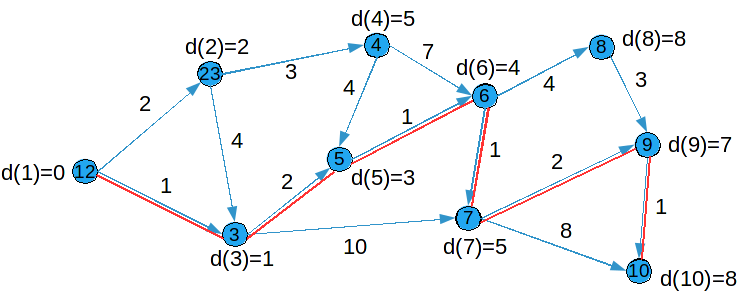
\includegraphics[height=5cm]{images/graph38.png}}

\section{Algoritmo Forward (grafi aciclici)}
\begin{enumerate}
	\item Poni $d(1)=0$ e $d(j)=\infty$, $\forall j\in V\setminus\{1\}$; sia $v=1$;
	\item Per ogni $j\in\Gamma(v)$ aggiorna:
	\begin{equation*}
		d(j)=min[d(j),d(v)+c_{vj}]
	\end{equation*}
	\item Se $v=n-1$ STOP, altrimenti poni $v=v+1$ e ritorna allo step 2.
\end{enumerate}

\textbf{Caso generale}: grafi orientati con cicli e costi degli archi $c_{ij}$ non-negativi.\\
Non si può applicare direttamente la ricorsione poichè è necessario imporre un ordine con cui calcolare la \ref{eq:4.1}.

\section{Algoritmo di Bellman}
Sia $D(k,j)$ il costo del cammino minimo da $s$ a $j$ contenente al più $k$ archi.\\
Si hanno due casi:
\begin{enumerate}
	\item Il cammino minimo di costo $D(k,j)$ contiene al più $k-1$ archi, quindi
	\begin{equation*}
		D(k,j)=D(k-1,j)
	\end{equation*}
	\item Il cammino minimo di costo $D(k,j)$ contiene $k$ archi, quindi
	\begin{equation}
		D(k,j)=\underset{i\in\Gamma^{-1}(j)}{min}[D(k-1,i),+c_{ij}] \label{eq:4.2}
	\end{equation}
\end{enumerate}
Partendo dalla \ref{eq:4.2} si a che la ricorsione è:
\begin{equation}
	D(k,j)=min[D(k-1,j),\underset{i\in\Gamma^{-1}(j)}{min}[D(k-1,i)+c_{ij}]] \label{eq:4.3}
\end{equation}
La ricorsione \ref{eq:4.3} impone un ordine implicito di calcolo:\\
prima $D(1,j),\ \forall j\in V$, poi $D(2,j)$, $D(3,j)$, \dots, $D(n-1,j)$.

\subsection{Schema dell'algoritmo cammini minimi da 1 ad ogni $\boldsymbol{j\in V}$}
\begin{enumerate}
	\item Definisci
	\begin{flalign*}
		& D(1,1)=0 \\
		& D(1,j)
		\begin{cases}
			c_{1j},\ \ \forall j\in\Gamma(1) \\
			\infty,\ \ \forall j\in V\setminus\Gamma(1)
		\end{cases}
	\end{flalign*}
	\item Per $k=2,\dots,n-1$ calcola
	\begin{equation*}
	D(k,j)=min[D(k-1,j),\underset{i\in\Gamma^{-1}(j)}{min}[D(k-1,i)+c_{ij}]],\ \ \ \ \forall j\in V
	\end{equation*}
	\item Poni $d(j)=D(n-1,j),\ \ \ \ \forall j\in V$
\end{enumerate}

\section{Knapsack 0-1}
Sono dati $n$ items ed un \textit{knapsack} di capacità $b$.\\
L'item $j$ ha peso $a_{j}$ e profitto $c_{j}$.\\
Si vuole riempire il knapsack massimizzando il profitto complessivo degli items caricati.\\
Assumiamo che i coefficienti $\{a_{j}\}$ e $b$ siano interi positivi
\begin{equation*}
	KP
	\begin{cases}
		z = max\sum_{j=1}^{n}c_{j}x_{j} \\
		\ \ \ \ \ \ \ \ \ \ \ \ \sum_{j=1}^{n}a_{j}b_{j}\le b \\
		\ \ \ \ \ \ \ \ \ \ \ \ x_{j}\in\{0,1\},\ \ j=1,\dots,n
	\end{cases}
\end{equation*}

\subsection{Esempio}
\begin{displaymath}
	\begin{cases}
		z=max 10x_{1}+7x_{2}+25x_{3}+24x_{4}\\
		\ \ \ \ \ \ \ \ \ \ \ \ \ 2x_{1}+1x_{2}+6x_{3}+5x_{4}\le 7 \\
		\ \ \ \ \ \ \ \ \ \ \ \ \ x_{j}\in\{0,1\},\ \ j=1,\dots,4
	\end{cases}
\end{displaymath}
La soluzione ottima è $x_{i}^{*}=1,\ x_{2}^{*}=0,x_{3}^{*}=0,x_{4}^{*}=1$.

\subsection{Osservazione 1}\label{ss:osservazione_1}
Se $x^{*}=(x_{1}^{*},x_{2}^{*},\dots,x_{n}^{*})$ è una soluzione ottima di $KP$ allora $(x_{1}^{*},x_{2}^{*},\dots,x_{k}^{*})$ con $k\le n$ è una soluzione ottima del seguente sottoproblema $KP_{k}(q)$.
\begin{equation*}
	KP_{k}(q)
	\begin{cases}
		f_{k}(q)=max\sum_{j=1}^{k}c_{j}x_{j}\\
		\ \ \ \ \ \ \ \ \ \ \ \ \ \ \ \ \ \sum_{j=1}^{k}a_{j}x_{j}\le q \\
		\ \ \ \ \ \ \ \ \ \ \ \ \ \ \ \ \ x_{j}\in\{0,1\},\ \ j=1,\dots,k \\
		\ \ \ \ \ \ \ \ \ \ \textnormal{dove }q=\sum_{j=1}^{k}a_{j}x_{j}^{*}
	\end{cases}
\end{equation*}
\subsubsection{Esempio}
$(x_{1}^{*}=1,x_{2}^{*}=0,x_{3}^{*}=0)$ deve essere la soluzione ottima del seguente problema
\begin{equation*}
	KP_{3}(q)
	\begin{cases}
		f_{3}(q)=max 10x_{1}+7x_{2}+25x_{3} \\
		2x_{1}+1x_{2}+6x_{3}\le q=2 \\
		x_{1},x_{2},x_{3}\in\{0,1\}
		\textnormal{dove }q=2x_{1}^{*}+1x_{2}^{*}+6x_{3}^{*}=2
	\end{cases}
\end{equation*}
La dimostrazione dell'\hyperref[ss:osservazione_1]{osservazione 1} è ovvia!\\
Si consideri la famiglia degli $n(b+1)$ sottoproblemi
\begin{equation*}
	\{KP_{k}(q):1\le k\le n,\ 0\le q\le b\}\ \ \ \ q\textnormal{ intero}
\end{equation*}
dove $q$ è detto 'stato' e $k$ è detto 'stadio'.\\
Il problema originario $KP$ è un membro di tale famiglia: $KP=KP_{n}(b)$ e $z=f_{n}(b)$ ($z$: costo ottimo di $KP$).\\

Come risolvere $KP_{k}(q)$ per un dato $k\le n$ e $q\le b$?

Sia $(x_{1}^{*},\dots,x_{k-1}^{*},x_{k}^{k})$ la soluzione ottima di $KP_{k}(q)$ di costo $f_{k}(q)$. Si hanno due casi:
\begin{enumerate}
	\item $x_{k}^{*}=0$, allora $q=\sum_{j=1}^{k}a_{j}x_{j}^{*}\equiv\sum_{j=1}^{k-1}a_{j}x_{j}^{*}$ e quindi $((x_{1}^{*},\dots,x_{k-1}^{*})$ è la soluzione ottima di $KP_{k-1}(q)$ ovvero $f_{k}(q)=f_{k-1}(q)$;
	\item $x_{k}^{*}=1$, allora $q=\sum_{j=1}^{k-1}a_{j}x_{j}^{*}+a_{k}$ e quindi $(x_{1}^{*},\dots,x_{k-1}^{*})$ è la soluzione ottima di $KP_{k-1}(q-ax)$ ovvero $f_{k}(q)=f_{k-1}(q-ax)+c_{k}$
\end{enumerate}
Se conosciamo $f_{k-1}(q)$ e $f_{k-1}(q-ax)$ si ha la seguente ricorsione:
\begin{equation*}
	f_{k}(q)=max[f_{k-1}(q),\ f_{k-1}(q-ax)+c_{k}]
\end{equation*}
Per calcolare $f_{k}(q)$, $\forall q$ per un dato $k$ dobbiamo conoscere i valori $f_{k-1}(q)$, $\forall q$.\\
Partiamo ponendo $f_{0}(q)=0$, per ogni $q$ tale che $0\le q\le b$. Ciò consente di calcolare $f_{1}(q)$, $\forall q$, mediante la ricorsione.\\
Quindi, $f_{1}(\cdot)$ consente di calcolare $f_{2}(\cdot),\dots$, infine, $f_{n-1}(\cdot)$ consente di calcolare $f_{n}(\cdot)$.
\subsubsection{Esempio}
\begin{equation*}
	\begin{cases}
	z=max 10_{1}+7x_{2}+25x_{3}+24x_{4}\\
	2x_{1}+1x_{2}+6x_{3}+5x_{4}\le 7 \\
	x_{j}\in\{0,1\},\ \ j=1,\dots,4
	\end{cases}
\end{equation*}
\begin{equation*}
	f_{k}(q)=max[f_{k-1}(q),f_{k-1}(q-a_{k})+c_{k}],\ \ \ \ \ \forall q\le b,\ \ k=b,\dots,n
\end{equation*}
\begin{table}[!h]
	\centering
	\begin{tabular}{l|llll}
		& $f_{1}$ & $f_{2}$ & $f_{3}$ & $f_{4}$ \\ \cline{1-5}
		$q=0$ & 0 & 0 & 0 & 0 \\
		$q=1$ & 0 & 7 & 7 & 7 \\
		$q=2$ & 10 & 10 & 10 & 10 \\
		$q=3$ & 10 & 17 & 17 & 17 \\
		$q=4$ & 10 & 17 & 17 & 17 \\
		$q=5$ & 10 & 17 & 17 & 24 \\
		$q=6$ & 10 & 17 & 25 & 31 \\
		$q=7$ & 10 & 17 & 32 & 34 \\
	\end{tabular}
\end{table}

Soluzione ottima:
\begin{flalign*}
	& fl_{4}(7)>f_{3}(7)\implies x_{4}^{*}=1 \\
	& fl_{3}(7-5)=f_{2}(2)\implies x_{3}^{*}=0 \\
	& fl_{2}(2)=f_{1}(2)\implies x_{2}^{*}=0 \\
	& fl_{1}(2)>f_{0}(2)\implies x_{1}^{*}=1 \\
\end{flalign*}

\subsection{Grafo dello spazio degli stati}
Alla ricorsione
\begin{equation*}
	f_{k}(q)=max[f_{k-1}(q),f_{k-1}(q-a_{k})+c_{k}],\ \ \ \ q\le b,\ \ k=1,\dots,n
\end{equation*}
si può associare un grafo aciclico $H=(X,A)$ così fatto:
\begin{itemize}
	\item $X$ si compone di $n+1$ partizioni $X_{0},X_{1},X_{2},\dots,X_{n}$.\\
	$X_{0}=(0)$ e ogni altra partizione $X_{k}$, $k=1,\dots,n$ contiene $b+1$ vertici corrispondenti agli stati $(0,1,2,\dots,b)$;
	\item Su ogni vertice $q\in X_{k}$ terminano al più due archi: l'arco avente vertice iniziale in $q-a_{k}\in X_{k-1}$ di costo $c_{k}$ (l'arco non esiste se $q\in X_{k-1}$ o se $q-a_{k}<0$)
\end{itemize}
\centerline{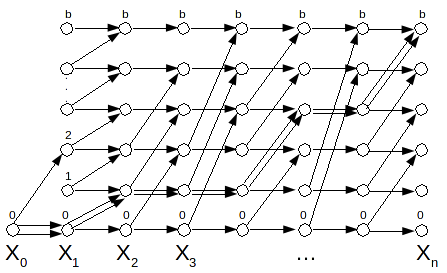
\includegraphics[height=5cm]{images/graph39.png}}
Il cammino di profitto massimo da $0\in X_{0}$ a $b\in X_{n}$ corrisponde a $f_{n}(b)$.
\subsection{Esempio}
\begin{equation*}
	\begin{cases}
		z=max\ 10x_{1}+7x_{2}+25x_{3}+24x_{4} \\
		2x_{1}+1x_{2}+6x_{3}+5x_{4}\le 7 \\
		x_{j}\in\{0,1\},\ \ j=1,\dots,4
	\end{cases}
\end{equation*}
\centerline{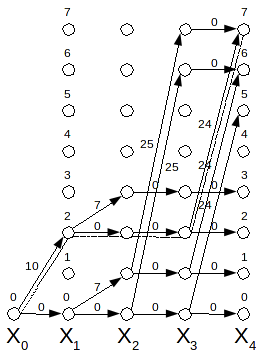
\includegraphics[height=8cm]{images/graph40.png}}
Non sono stati disegnati gli archi inutili, ovvero, non attraversabili da alcun cammino che parte da $0\in X_{0}$.\\
Il grafo mostra che è inutile calcolare $f_{1}(q)$, $q\in\{1,3,4,5,6,7\}$ ma anche $f_{2}(q)$, $q=4,\dots,7$, etc.\\\\
Qual è un algoritmo migliore per implementare la ricorsione per il knapsack 0-1?

\subsection{Ricorsione Froward - Knapsack 0-1}
\begin{enumerate}
	\item Poni $f_{0}(0)=0$ e $f_{0}(q)=-\infty$, $q=1,\dots,b$. Sia $k=0$;
	\item inizializza $f_{k+1}(q)=-\infty$, $q=0,1,\dots,b$;
	\item Per ogni $q=0,1,\dots,b$ tale che $f_{k}(q)\ge 0$ aggiorna 
	\begin{equation*}
		f_{k+1}(q)=max\ [f_{k+1}(q),f_{k}(q)] 
	\end{equation*}
	se $q+a_{k+1}\le b$ allora
	\begin{equation*}
		f_{k+1}(q+a_{k+1})=max\ [f_{k+1}(q+a_{k+1}),f_{k}(q)+c_{k+1}]
	\end{equation*}
	\item Se $k=n-1$ \textit{STOP}, altrimenti poni $k=k+1$ e ritorna allo step 2.
\end{enumerate}

\section{Programmazione a numeri interi}
\begin{flalign*}
	& F^{*}=Min\ \sum_{j=1}^{n}C_{j}x_{j} \\
	& \ \ \ \ \ \ \ \ \ \ \ \ \ \ \ \sum_{j=1}^{n}a_{1j}x_{j}=b_{1} \\
	& \ \ \ \ \ \ \ \ \ \ \ \ \ \ \ \sum_{j=1}^{n}a_{2j}x_{j}=b_{2} \\
	& \ \ \ \ \ \ \ \ \ \ \ \ \ \ \ \ \ \ \vdots\ \ \ \ \ \ \ \vdots \\
	& \ \ \ \ \ \ \ \ \ \ \ \ \ \ \ \sum_{j=1}^{n}a_{mj}x_{j}=b_{m} \\
	& \ \ \ \ \ \ \ \ \ \ \ \ \ \ \ x_{j}\ge 0 \textnormal{ e intero}
\end{flalign*}
Per semplicità assumiamo che
\begin{flalign*}
	& a_{ij}\ge 0\ \ \ \ \ \ \ \forall i,j \\
	& \ \,b_{i}\ge 0\ \ \ \ \ \ \;\forall i
\end{flalign*}

\section{Programmazione Dinamica}
\begin{flalign*}
	& F_{k}(\ubar{v})=Min\ \sum_{j=1}^{k}C_{j}x_{j} \\
	& \ \ \ \ \ \ \ \ \ \ \ \ \ \ \ \ \ \ \sum_{j=1}^{k}a_{1j}x_{j}=v_{1} \\
	& \ \ \ \ \ \ \ \ \ \ \ \ \ \ \ \ \ \ \sum_{j=1}^{k}a_{2j}x_{j}=v_{2} \\
	& \ \ \ \ \ \ \ \ \ \ \ \ \ \ \ \ \ \ \ \ \vdots\ \ \ \ \ \ \ \vdots \\
	& \ \ \ \ \ \ \ \ \ \ \ \ \ \ \ \ \ \ \sum_{j=1}^{k}a_{mj}x_{j}=v_{m} \\
	& \ \ \ \ \ \ \ \ \ \ \ \ \ \ \ \ \ \ x_{1},x_{2},\dots,x_{k}\ge 0 \textnormal{ e intero}
\end{flalign*}
$F_{k}(V)$ venga calcolato per $k=1,\dots,n$; $\forall \ubar{v}\le \ubar{b}$ e $\ubar{v}\ge 0$.\\
La soluzione ottima è data da
\begin{equation*}
	F^{*}=F_{n}(\ubar{b})
\end{equation*}

\section{Ricorsione di Programmazione Dinamica}
Le funzioni $F_{k}(\ubar{v})$ si possono calcolare come segue:
\begin{equation*}
	F(\ubar{v})=Min\ \{F_{k-1}(\ubar{v}),\ \underset{\underset{x_{k}\ intero}{x_{k}>0}}{Min}[F_{k-1}(\ubar{v}-a^{k}x_{k})+c_{k}x_{k}]\})
\end{equation*}
per $k=1,\dots,n$; $\forall \ubar{v}\le \ubar{b}$.\\
La ricorsione richiede di conoscere $F_{0}(\ubar{v})$
\begin{equation*}
	F_{0}(\ubar{v})
	\begin{cases}
		0 \textnormal{ per }v={0}\\
		\infty \textnormal{ per ogni } 0 < \ubar{v}\le b
	\end{cases}
\end{equation*}
$k$ rappresenta lo \textbf{stadio} della ricorsione mentre $v$ è la \textbf{variabile di stato}.

\section{Programmazione Dinamica: il TSP}
È dato un grafo $G=(X,A)$ di $n=|X|$ vertici ed $m=|A|$ archi. Ad ogni arco $(x_{i},x_{j})\in A$ è associato un costo $c_{ij}$.

Determinare il cammino di costo minimo che parte da $x_{1}$, attraversa tutti i vertici di $G$ una ed una sola volta e termina in $x_{1}$.
\begin{itemize}
	\item[] $f(S,x_{i})$: costo minimo di un cammino che parte da $x_{i}$, attraversa tutti i vertici di $S\in X\setminus{x_{i}}$ una ed una sola volta e termina in $x_{i}\in S$.
\end{itemize}

\subsection{Ricorsione per il calcolo di $\boldsymbol{f(S,x_{i})}$}
\begin{equation*}
	f(S,x_{i})=\underset{x_{j}\in S\setminus{x_{i}}}{Min}\{f(S\setminus{x_{i}},x_{j})+c_{ji}\}
\end{equation*}
Le $f(S,x_{i})$ vanno calcolate:
\begin{equation*}
	\forall S\subseteq X \textnormal{ tale che }x_{1}\in S,\ |S|\ge 2,\ \forall x_{i}\in S\setminus{x_{1}}
\end{equation*}
\subsubsection{Calcolo del valore $\boldsymbol{z^{*}}$ della soluzione ottima}
\begin{equation*}
	z^{*}=\underset{x_{i}\in X\setminus{X_{1}}}{Min}\{f(X,x_{i})+c_{i1}\}
\end{equation*}
È richiesta la seguente inizializzazione:
\begin{equation*}
	f(\{x_{1}\},x_{1})=0
\end{equation*}
\clearpage
\subsection{Considerazioni computazionali}
Il calcolo di $f(S,x_{i})$ richiede di conoscere il valore di $f(S\setminus\{x_{i}\}, x_{j})$ $\forall x_{j}\in S\setminus\{x_{i}\}$\\\\
\textbf{Esempio:} calcolo di $f(\{x_{2},x_{3},x_{4}x_{5}\},x_{2})$
\begin{equation*}
	f(\{x_{2},x_{3},x_{4}x_{5}\},x_{2})=\underset{x_{j}\in\{x_{3},x_{4},x_{5}\}}{Min}[f(\{x_{3},x_{4},x_{5}\},x_{j})+c_{j2}]
\end{equation*}
e quindi bisogna conoscere:
\begin{equation*}
	f(x_{3},x_{4}x_{5}\},x_{3});\ \ f(\{x_{3},x_{4}x_{5}\},x_{4});\ \ f(\{x_{3},x_{4}x_{5}\},x_{5})
\end{equation*}

Le \textbf{variabili di stato} sono rappresentate da
\begin{equation*}
	(S,x_{i});\ \ \ \ \forall\ S\subseteq X\setminus\{x_{i}\},\ \ \forall\ X_{i}\in S
\end{equation*}
Lo stadio può essere definito in modi diversi; deve corrispondere al sequente principio:\\

"se lo stato $(S,x_{i})$ è associato allo stadio $K$ allora ognuno degli stati $(S\setminus\{x_{i}\},x_{j})$ deve essere associato ad uno stadio $K^{'}<K^{''}$."\\

\textbf{Ad esempio:} stadio: $|S|$ cardinalità di S.\\
È ovvio che allo stadio 1 vengono calcolate le $f(S,x_{i})$ $\forall\ S$ per cui $|S|=1$.\\
Allo stadio 2 si calcola $f(S,x_{i})$, $\forall\ S$ per cui $|S|=2$.\\
\vdots\\
Allo stadio k si calcola $f(S,x_{i})$, $\forall\ S$ per cui $|S|=k$ e quindi sono note le $f(S\setminus\{x_{i}\},x_{j})$ in quanto sono state calcolate allo stadio $k-1$.\\

Lo stadio può essere definito diversamente:
\begin{itemize}
	\item Si associ un peso $q_{i}\ge 1$ ad ogni $x_{i}\in X$. Si assegni ad ogni stato $(S,x_{i})$ allo stadio $\sum_{i\in S}^{q_{i}}$. In tal modo gli stati vengono suddivisi in $\sum_{i=1}^{n}q_{i}$ stadi;
	\item si noti che questa definizione è corretta, infatti dato lo stato $(S,x_{i})$ corrispondente a $\sum_{i\in S}q_{i}=q(S)$ ogni stato $(S\setminus\{x_{i},x_{j}\})$ corrisponde allo stadio $q(S)-q_{i}$.
\end{itemize}
È banale notare che ponendo $q_{i}=1$, $\forall\ x_{i}\in X$ lo stadio corrisponde alla cardinalità di $S$ (come visto in precedenza).

\subsection{Esempio del TSP con 5 città}
$[c_{ij}]=
	\begin{bmatrix}
		- & 6 & 11 & 3 & 4 \\
		7 & - & 14 & 8 & 10 \\
		12 & 5 & - & 10 & 2 \\
		6 & 15 & 7 & - & 5 \\
		4 & 9 & 8 & 13 & 6 -
	\end{bmatrix}$\\
	
Applichiamo la ricorsione:
\begin{equation*}
	f(S,x_{i})=\underset{x_{j}\in S\setminus\{x_{i}\}}{Min}\{f(S\setminus\{x_{i},x_{j}\})+c_{ji}\}
\end{equation*}
Inizializzazione:
\begin{equation*}
	f(\{x_{i}\},x_{i})=c_{1i};\ \ \ \ \forall\ x_{i}\in X\setminus\{x_{1}\}
\end{equation*}
\begin{flalign*}
	& f(\{2\},2)=6\\
	& f(\{3\},3)=11\\
	& f(\{4\},4)=3\\
	& f(\{5\},5)=4\\
\end{flalign*}

\subsubsection{Stadio 2: Calcolo $\boldsymbol{f(S,x_{i}),\ \forall\ S\subset X\setminus\{x_{i},\ s.t.\ |S|=2;\ \forall\ x_{i}\in S\}}$}
\begin{flalign*}
	& f(S,x_{i})=\underset{x_{j}\in S\setminus\{x_{j}\}}{Min}\{f(S\setminus\{x_{i}\},x_{j})+c_{ji}\} \\\\
	& f(\{2,3\},2)=f(\{3\},3)+c_{3,2}=11+5=16 \\
	& f(\{2,3\},3)=f(\{2\},2)+c_{2,3}=6+14=20 \\\\
	& f(\{2,4\},2)=f(\{4\},4)+c_{4,2}=3+15=18 \\
	& f(\{2,4\},3)=f(\{2\},2)+c_{2,4}=6+8=14 \\\\
	& f(\{2,5\},2)=f(\{5\},5)+c_{5,2}=4+9=13 \\
	& f(\{2,5\},3)=f(\{2\},2)+c_{2,5}=6+10=16 \\
\end{flalign*}
Similarmente:
\begin{flalign*}
	& f(\{3,4\},3)=10 \\
	& f(\{3,4\},4)=21 \\\\
	& f(\{3,5\},3)=12 \\
	& f(\{3,5\},5)=13 \\\\
	& f(\{4,5\},4)=17 \\
	& f(\{4,5\},5)=8 \\\\
\end{flalign*}
\subsubsection{Stadio 3: $\boldsymbol{f(S,x_{i}),\ \forall\ S\subset X\setminus\{x_{i},\ s.t.\ |S|=3;\ \forall\ x_{i}\in S\}}$}
\begin{flalign*}
	& f(\{2,3,4\},2)=\underset{x_{j}\in\{3,4\}}{Min}\{f(\{3,4\},x_{j})+c_{j2}\}\\\\
	& f(\{2,3,4\},2)=Min\ \{f(\{3,4\},3)+c_{3,2};\ f(\{3,4\},4)+c_{4,2}\}=Min\ \{10+5;\ 21+15\}=15 \\
	& f(\{2,3,4\},3)=Min\ \{f(\{2,4\},2)+c_{2,3};\ f(\{2,4\},4)+c_{4,3}\}=Min\ \{18+4;\ 14+7\}=21 \\
\end{flalign*}
Similarmente:
\begin{flalign*}
	& f(\{2,3,4\},4)=24 \\\\
	& f(\{2,3,5\},2) = 17;\ \ \ \ \ f(\{2,3,5\},3)=24;\ \ \ \ \ f(\{2,3,5\},5)=22 \\
	& f(\{2,4,5\},2) = 17;\ \ \ \ \ f(\{2,4,5\},4)=21;\ \ \ \ \ f(\{2,4,5\},5)=19 \\
	& f(\{3,4,5\},3) = 16;\ \ \ \ \ f(\{3,4,5\},4)=22;\ \ \ \ \ f(\{3,4,5\},5)=12 \\
\end{flalign*}
\subsubsection{Stadio 4}
\begin{equation*}
	f(\{2,3,4,5\},2)=\underset{x_{j}\in\{3,4,5\}}{Min}\{f(\{3,4,5\},x_{j})+c_{j2}\}
\end{equation*}
da cui
\begin{flalign*}
	& f(\{2,3,4,5\},2)=Min\ \{f(\{3,4,5\},3)+c_{3,2},\ f(\{3,4,5\},4)+c_{4,2},\ f(\{3,4,5\},5)+c_{5,2}\} = \\
	& \qquad\qquad\qquad\qquad Min\{16+5;\ 22+15;\ 12+9\}=21
\end{flalign*}
Similarmente
\begin{flalign*}
	& f(\{2,3,4,5\},3)=27 \\
	& f(\{2,3,4,5\},4)=25 \\
	& f(\{2,3,4,5\},5)=23 \\
\end{flalign*}
\subsubsection{Soluzione ottima}
\begin{flalign*}
	& z^{*}=\underset{x_{j}\in\{2,3,4,5\}}{Min}\{f(\{2,3,4,5\},x_{i})+c_{i1}\}= \\
	& \ \ \ =\{21+7;\ 27+12;\ 25+6;\ 23+4\}=27
\end{flalign*}

\newpage
\subsubsection{Spazio degli stati del TSP}
\begin{figure}[h]
	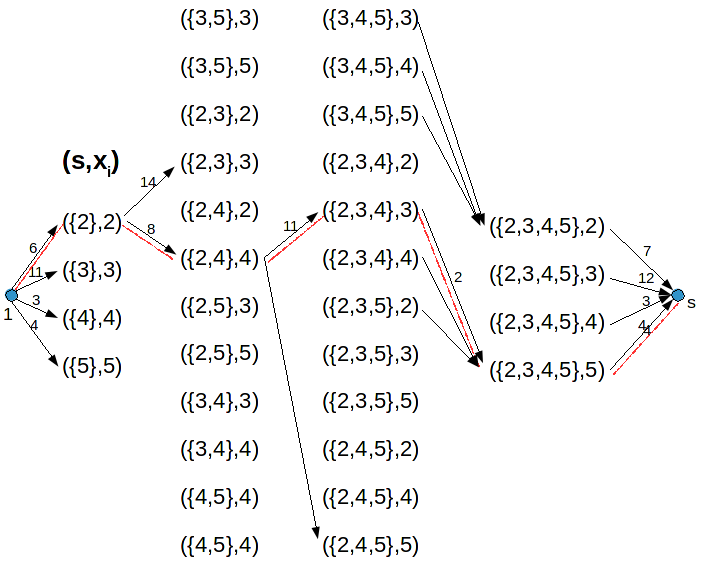
\includegraphics[height=14cm]{images/graph41.png}
	\caption{Solo alcuni degli archi sono raffigurati}
\end{figure}

\section{Ricorsione Forward per il TSP}
\begin{enumerate}
	\item $\mathscr{L}_{0}=\{(\{1\},1)\}$, $f(\{1\},1)=0$, $p(\{1\},1)=0$. Inizializza $\mathscr{L}_{r}=\emptyset$, $r=1,\dots,n$. Definisci $k=1$.
	\item Espansione degli stati del set $\mathscr{L}_{k-1}$: per ogni stato $(S,i)\in\mathscr{L}_{k-1}$ ripeti lo step 3.
	\item Genera/Aggiorna gli stati di $\mathscr{L}_{k}$ raggiungibili da $(S,i)$: per ogni vertice $j\in\Gamma_{i}\setminus S$ considera lo stato $(S',i)$, dove $S'=S\cup\{j\}$, che si ottiene aggiungendo l'arco $(i,j)$.\\
	Il costo di $(S',j)$ è $h=f(S,i)+c_{ij}$.\\
	Si hanno i seguenti casi:
	\begin{itemize}
		\item $(S',j)\in\mathscr{L}_{k}$, allora $\mathscr{L}_{k}=\mathscr{L}_{k}\cup \{f(S',j)\}$ e $f(S',j)=h$. Poni $p(S',j)=(S,i)$;
		\item $(S',j)\in\mathscr{L}_{k}$ ma $f(S',j)>h$, allora $f(S',j)=h$ e $p(S',j)=(S,i)$.
	\end{itemize}
	\item Poni $k=k+1$; se $k\le n$ vai allora step 2.
	\item Il costo ottimo $z^{*}$ del TSP si ottiene come segue:
	\begin{equation*}
		z^{*}=\underset{(X,j)\in\mathscr{L}_{n}}{Min}[f(X,j)+c_{j1}]
	\end{equation*}
\end{enumerate}

\section{Taglio 2-dimesionale a ghigliottina}
\centerline{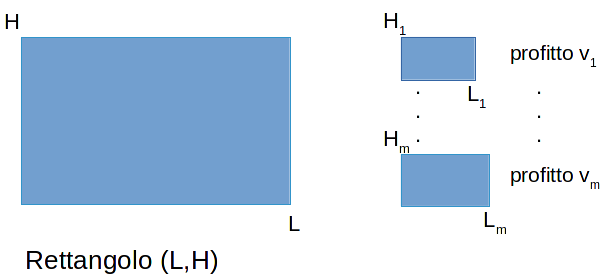
\includegraphics[height=6cm]{images/shape1.png}}
\begin{itemize}
	\item Il rettangolo e i pezzi hanno dimensioni intere e non possono essere ruotati;
	\item Sono ammessi solo tagli a ghigliottina;
	\item Ogni tipo di pezzo è disponibile in quantità illimitata
\end{itemize}

\textbf{Obiettivo}: massimizzare il profitto totale dei pezzi tagliati.

\begin{figure}[h]
	\centering
	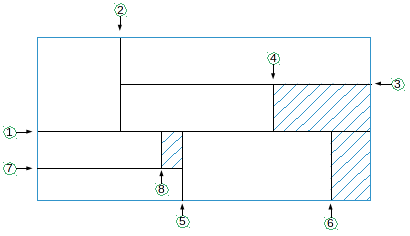
\includegraphics[height=5cm]{images/shape2.png}
	\caption{Esempio di taglio a ghigliottina}
\end{figure}
Indichiamo con:\\

$F(x,y)$ il profitto massimo per tagliare un rettangolo di dimensione $(x,y)$ con $x\le L$ e $y\le H$.\\
$F(L,H)$ il valore della soluzione ottima.

\clearpage
\subsection{Calcolo di $\boldsymbol{F(x,y)}$}
Si hanno tre casi:
\begin{enumerate}
	\item Il rettangolo $(x,y)$ contiene al più un pezzo (o nessuno) $F(x,y)=max\ [0,\ v{i}:\ l_{i}\le x,\ h_{i}\le y,\ i=1,\dots,m]$
	\item Il rettangolo $(x,y)$ contiene due o più pezzi che per essere tagliati richiedono almeno un taglio a ghigliottina o parallelo alla lunghezza in posizione $\beta$ parallelo all'altezza in posizione $\alpha$.
	\centerline{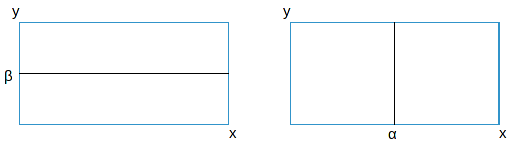
\includegraphics[height=4cm]{images/shape3.png}}
	$F(x,y)=F(x,\beta)+F(x,y-\beta)$ o $F(x,y)=F(\alpha,y)=F(x-\alpha,y)$
\end{enumerate}

\subsection{Inizializzazione}
Per ogni $x=1,...,L$ e $y=1,\dots,H$ poni
\begin{equation*}
	F^{0}(x,y)=max\ [0,\ v_{i}:\ l_{i}\le x,\ h_{i}\le y,\ i=1,\dots,m]
\end{equation*}
\begin{itemize}
	\item se $F^{0}(x,y)=v_{i^{*}}$ poni $X-cut(x,y)=l_{i^{*}}$ e $Y-cut(x,y)=h_{i^{*}}$
	\item se $F^{0}(x,y)=0$ poni $X-cut(x,y)=Y-cut(x,y)=0$
\end{itemize}
La ricorsione: per ogni $x=1,\dots,L$ e $y=1,\dots,H$ calcola
\begin{equation*}
	F(x,y)=max\ [F^{0}(x,y);\ F(x,\beta)+F(x,y-\beta),\ \beta=1,\dots,y-1,\ F(\alpha,y)+F(x-\alpha,y),\ \alpha=1,\dots,x-1]
\end{equation*}
\begin{itemize}
	\item se $F(x,y)=F(x,\beta^{*})+F(x,y-\beta^{*})$ per qualche $\beta^{*}$ poni\\ $X-cut(x,y)=0$ e $Y-cut(x,y)=\beta^{*}$
	\item se $F(x,y)=F(\alpha^{*},x)+F(x-\alpha^{*},y)$ per qualche $\alpha^{*}$ poni \\$X-cut(x,y)=\alpha^{*}$ e $Y-cut(x,y)=0$
\end{itemize}
Si può migliorare la ricorsione sostituendo
\begin{flalign*}
	& \beta=1,\dots,y-1\textnormal{ con }1\le\beta\le y/2 \\
	& \alpha=1,\dots,x-1\textnormal{ con }1\le\alpha\le x/2
\end{flalign*}
\subsection{Esempio}
Sia $y=5$
\begin{flalign*}
	F(x,5)=max\ [F^{0}(x,5),\ \overbrace{F(x,1)+F(x,4)}^{T_{1}},\overbrace{F(x,2)+F(x,3)}^{T_{2}},\underbrace{F(x,3)+F(x,2)}_{T_{3}},\underbrace{F(x,4)+F(x,1)}_{T_{4}},\dots]
\end{flalign*}
Si noti che $T_{1}\equiv T_{4}$ e $T_{2}\equiv T_{3}$ è ciò giustifica la sostituzione di $\beta=1,\dots,y-1$ con $1\le\beta\le y/2$.

Complessità: $O(L\cdot H(L+H))$.

\subsection{Normal Cuts}
Riduce la complessità in molte situazioni reali.
\begin{figure}[h]
	\centering
	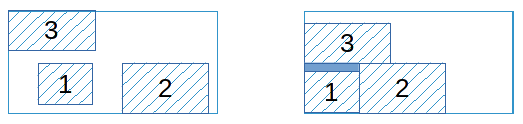
\includegraphics[height=2.0cm]{images/shape4.png}
	\caption{Sono equivalenti}
\end{figure}

I pezzi possono essere spostati in basso e a sinistra fino a che il lato sinistro e il lato inferiore di ogni pezzo sono adiacenti ad un taglio o al lato sinistro e inferiore del rettangolo.\\
I tagli a ghigliottina possono avvenire solo nelle seguenti posizioni.

\textbf{Posizioni possibili per tagli paralleli all'altezza}
\begin{equation}
	L_{0}=(x:\ x=\sum_{i=1}^{m}l_{i}\xi_{i},\ 1\le x\le L,\ \xi\ge 0 intero)\ \ \ U(L)
\end{equation}
\textbf{Posizioni possibili per tagli paralleli alla lunghezza}
\begin{equation}
		H_{0}=(y:\ y=\sum_{i=1}^{m}h_{i}\xi_{i},\ 1\le y\le H,\ \xi\ge 0 intero)\ \ \ U(H)
\end{equation}
Definiamo
\begin{flalign*}
	& p(x)=max\ [0,\ \alpha:\alpha\le x,\ \alpha\in L_{0}],\ \ x=1,\dots,L-1 \\
	& p(y)=max\ [0,\ \beta:\beta\le y,\ \beta\in H_{0}],\ \ y=1,\dots,H-1
\end{flalign*}
La ricorsione diviene, per ogni $x=1,\dots,L$ e $y=1,\dots,H$:
\begin{flalign*}
	& F(x,y)=max\ [F^{0}(x,y);\ F(x,\beta)+F(x,q(y-\beta)),\ \beta\in H_{0},\ \beta\le y/2,\\ 
	&\qquad\qquad\qquad\ \ \  F(\alpha,y)+F(p(x-a),y),\ \alpha\in L_{0},\ \alpha\le x/2]
\end{flalign*}

\section{Rilassamento dello spazio degli stati}
In molti casi lo spazio degli stati su cui è definita una ricorsione di programmazione dinamica (DP) ha dimensioni proibitive (si veda il caso del TSP).

\subsection{Come ridurre lo spazio degli stati}
\begin{enumerate}
	\item Eliminare stati che non possono condurre ad alcuna soluzione ottima.\\
	Ad esempio usando un lower bound.
	\item Riducendo in modo euristico gli stati fino a che lo spazio risultante non ha dimensioni "accettabili".\\
	Ad esempio scegliendo mediante qualche regola un sottoinsieme limitato di stato ad ogni stadio. Lo spazio risultante potrebbe non contenere la soluzione ottima.
	\item Contraendo più stati in un unico stato in modo che la ricorsione di $DP$ nello spazio rilassato produca un lower bound (questo metodo è noto: \textit{state space relaxation}).
\end{enumerate}

Vedremo come il metodo state space relaxation fornisca un lower bound da usare al punto 1.

\subsection{Lower bound al cammino minimo}
Il metodo della \textbf{State Space Relaxation} si basa sulla sequente semplice idea che consente di calcolare un lower bound al costo del cammino minimo in un grafo.
\begin{figure}[!h]
	\centering
	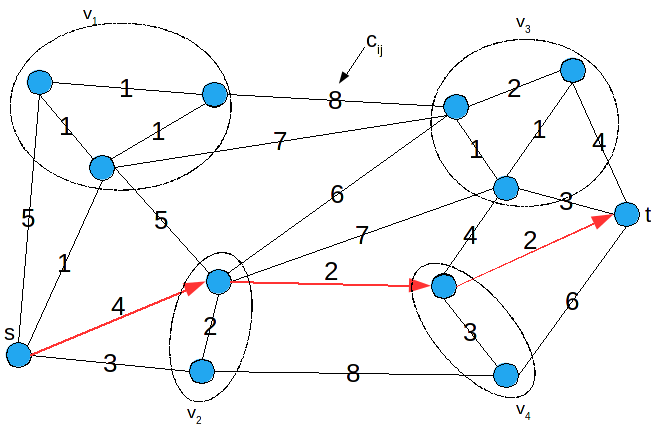
\includegraphics[height=7cm]{images/graph42.png}
	\caption{Il costo del cammino del grafo $G=(X,A)$ da $s$ a $t$ è 8}
\end{figure}

I vertici sono clusterizzati in 4 cluster come mostrato (non è importante il criterio di clustering per quanto segue).\\
Ogni $v_{k}\subset X$, $k=1,\dots,4$ e $v_{k}\cap V_{j}=\emptyset$ $j\neq k=1\,dots,4$.

\clearpage
\textbf{Grafo rilassato $\boldsymbol{\bar{G}=(\bar{X,\bar{A}}):\ \bar{X}=\{v_{0},v_{1},\dots,v_{4},v_{5}\}}$}
\begin{table}[!h]
	\begin{tabular}{m{11cm} m{5cm}}
		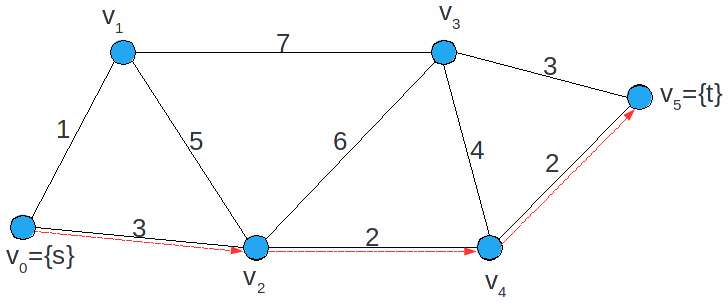
\includegraphics[height=5cm]{images/graph43.png} & \begin{equation*}
			\bar{c_{ij}}=\underset{\underset{s\in V_{j}}{r\in _V{i}}}{min}[c_{rs}]
		\end{equation*}
	\end{tabular}
\end{table}

Il costo del cammino minimo da $v_{0}$ a $v_{5}\in\bar{G}$ ($ =7$) è un valido lower bound.

\subsubsection{Esempio}
\begin{figure}[!h]
	\centering
	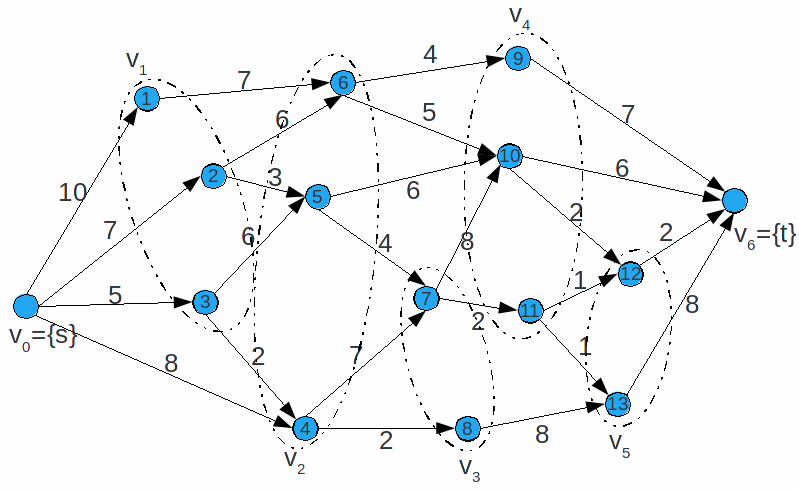
\includegraphics[height=6cm]{images/graph44.png}
\end{figure}
Nel caso di un grafo aciclico, come nell'esempio, può essere conveniente che ogni cluster $v_{k}$ sia tale che $\forall\ j,j\in v_{k}(i<j)$ non esista l'arco $(i,j)$ in A.

\textbf{Grafo rilassato}\\
\begin{figure}[H]
	\centering
	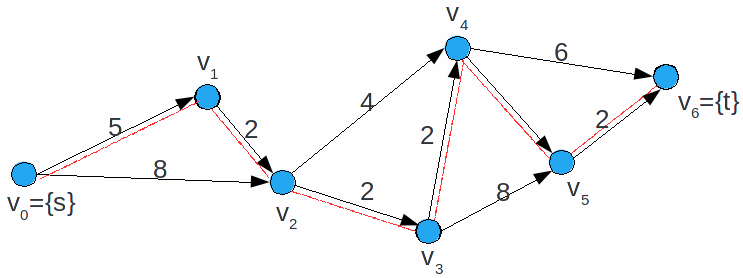
\includegraphics[height=4cm]{images/graph45.png}
\end{figure}

\subsection{Sitema discreto multistadio}
$s=(s_{1},\dots,s_{m})$: variabile di stato

$\mathscr{L}_{k}$: insieme degli stati allo stadio k

$f_{k}(s)$ è il costo minimo per cambiare lo stato del sistema dallo stato iniziale (allo stadio $0$) allora stato $s\in\mathscr{L}_{k}$ allora stadio $k$
\begin{equation*}
	f_{k}(s)=\underset{s'\in\Delta^{-1}(s)}{min}[f_{k-1}(s')+v(s',s)],\ \ \ \ \forall\ s\in\mathscr{L}_{k}
\end{equation*}
dove $\Delta^{-1}(s)$ sono gli stati che raggiungono lo stato $s$ e $v(s',s)$ è il costo per cambiare il sistema dallo stato $s'$ allo stato $s$.

\subsubsection{Esempio: il TSP}
\begin{equation*}
	f(s,i)=\underset{j\in S\setminus\{i,1\}}{min}[f(S\setminus\{i\},j)+c_{ji}],\ \ \ \ |S|\ge 2
\end{equation*}
Definiamo (ad esempio)
\begin{flalign*}
	 & s=(S,i)                                                              \\
	 & \mathscr{L}_{k}=\{(S,i): S\subset X\ t.c.\ 1\in S,\ |S|=k,\ i\in S\} \\
	 & \Delta^{-1}(S,i)=\{(S\setminus\{i\},j):\ j\in S\{i,1\}\}             \\
	 & v((S\setminus\{i\},j),(S,i))=c_{ji}
\end{flalign*}
Sia $g(\cdot)$ una funzione di "mapping" dallo spazio degli stati $\mathscr{L}$ allo spazio ridotto $R$.\\
\centerline{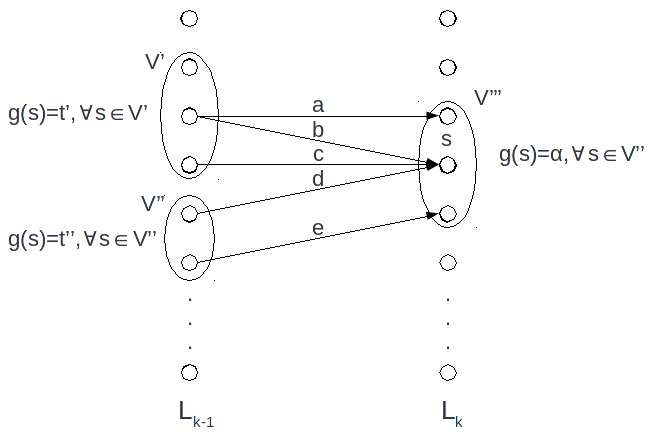
\includegraphics[height=6.1cm]{images/graph46.png}}

Più stati di $\mathscr{L}$ vengono associati ad un unico stato di $R$.

Per ogni $s'\in\Delta^{-1}(s)$ esiste l'arco $(g(s'),g(s))$.

$F^{-1}(\alpha)$: predecessori di $\alpha\in R$ (ad esempio: $F^{-1}(\alpha)=\{t',t''\}$).

$\bar{v}(\alpha,\beta)$: $min[v(s',s):\forall s',s\in\mathscr{L}\ t.c.\ g(s')=\alpha\ e\ g(s)=\beta]$.\\

\textbf{Esempio}\\

$\bar{v}(t',\alpha)=min[a,b,c]$, $\bar{v}(t'',\alpha)=min[d,e]$\\

Nello spazio $R$ la ricorsione diviene
\begin{equation*}
	f_{k}(g(s))=\underset{t\in F^{-1}(g(s))}{min}[f_{k-1}(t)+\bar{v}(t,g(s))]
\end{equation*}
Si noti che $f_{k}(g(s))\le f_{k}(s)$, $\forall\ s\in\mathscr{L}$, ovvero, $f_{k}(g(s))$ è un lower bound a $f_{k}(s)$.\\
La funzione $g(\cdot)$ deve essere tale per cui
\begin{enumerate}
	\item $p^{-1}(\alpha)$ può essere calcolato facilmente $\forall\alpha\in R$
	\item $\bar{v}(\alpha,\beta)$ può essere calcolato facilmente o approssimato con un lower bound
\end{enumerate}

\subsection{Rilassamento dello spazio degli stati per il TSP}
\begin{equation*}
	f(s,i)=\underset{j\in S\setminus{i,1}}{min}[f(S\setminus{i},j)+c_{ji}],\ \ |S|\ge 2
\end{equation*}
$(s,i)$: variabile di stato\\

Funzione di mapping: $(s,i)\rightarrow (g(s),i)$
\begin{flalign*}
	& \Delta^{-1}(s,i)=\{(S\setminus{i},j):\ j\in S\setminus\{i,1\}\} \\
	& F^{-1}(g(s),i)=\{(g(S\setminus\{i\}),j):\ j\in S\setminus\{i,1\}\}\subseteq\{g(S\setminus\{i\},j):\ j\in \Gamma^{-1}\} \\
	& v((S\setminus\{i\},j)), (s,i))=c_{ji}
\end{flalign*}
quindi $v()$ non dipende da $S$, per cui
\begin{equation*}
	\bar{v}((g(S\setminus\{i\}),j),(g(s),i))=c_{ji}
\end{equation*}
La ricorsione nello spazio rilassato diviene
\begin{equation*}
	f(g(s),i)=\underset{j\in\Gamma^{-1}\setminus\{1\}}{min}[f(g(S\setminus\{i\}),j)+c_{ji}],\ \ \ |S|\ge 2
\end{equation*}
Inizializzazione
\begin{equation*}
	f(g(\{1,i\}),i)=c_{1j},\ \ \forall\ i
\end{equation*}

\clearpage
\subsection{Funzioni di mapping $\boldsymbol{g(\cdot)}$ per il TSP}
\subsubsection{Rilassamento \textit{n-path}}
$g(S)=|S|:\ (S,i)\rightarrow(k,i)$ dove $k=|S|$
\begin{equation*}
	f(k,i)=\underset{j\in\Gamma^{-1}_{i}\setminus\{1\}}{min}[f(k-1,j)+c_{ji}],\ \ k\ge 2
\end{equation*}
Inizializza $f(1,i)=c_{1i}$, $\forall\ i$

$f(k,1)$: cammino minimo di cardinalità $k$ da 1 a $i$ (tale cammino può essere non elementare).

$z^{*}=\underset{i}{min}[f(n-1,i)+c_{i1}]$ è un lower bound al $TSP$

\begin{table}[!h]
	\begin{tabular}{m{8cm} m{5cm}}
		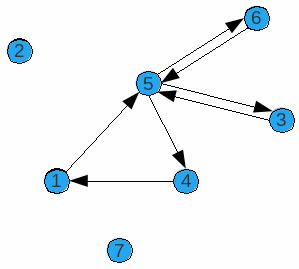
\includegraphics[height=6cm]{images/graph47.png} & Il vertice 5 è visitato 3 volte.\newline I vertici 2 e 7 non sono visitati.
	\end{tabular}
\end{table}
\textbf{Miglior lower bound}\\
Si penalizzi in modo Lagrangiano i vertici non visitati esattamente una ed una sola volta.

\clearpage
\subsection{Rilassamento q-path}
Ad ogni vertice $i$ si associ un peso $q_{i}\le 1$ e $q_{1}=0$
\begin{equation*}
	g(S)=\sum_{i\in S}q_{i}:\ (S,i)\rightarrow(q,i)\textnormal{ dove }q=\sum_{i\in S}q_{i}
\end{equation*}
\begin{equation*}
	f(q,i)=\underset{j\in\Gamma^{-1}_{i}\setminus\{1\}}{min}[f(q-q_{i},j)+c_{ji}],\ q>q_{i}
\end{equation*}
Inizializza:
\begin{flalign*}
	&f(q,i)=
	\begin{cases}
		c_{1i}, \textnormal{ se }q=q_{i} \\
		\infty, \textnormal{ altrimenti}
	\end{cases}
	,\ \ \forall i \textnormal{ e }\forall\ q=1,\dots,Q \\
	& \textnormal{dove }Q=\sum_{i=1}^{k}q_{i}
\end{flalign*}
Il lower bound al $TSP$ è dato da
\begin{equation*}
	z^{*}=\underset{i}{min}[f(Q,i)+c_{j1}]
\end{equation*}
Il cammino di costo $f(q,i)$ può essere non elementare e quindi anche il circuito corrispondente a $z^{*}$.\\
Un miglior lower bound, anche in questo caso, si ottiene mediante un ascent lagrangiano in cui vengono penalizzati i vertici non visitati esattamento una sola volta.

\subsection{Eliminazione dei loops di 2 vertici}
Sia $f(k,1)$ che $f(q,i)$ possono produrre cammini non elementari con loops di 2 vertici (vedi esempio)

\centerline{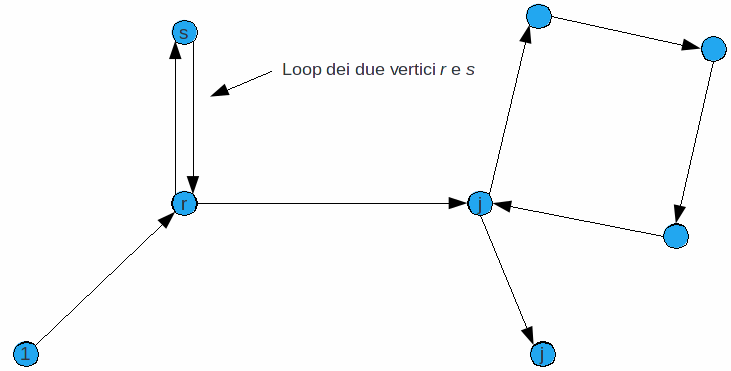
\includegraphics[height=5cm]{images/graph48.png}}
I loops di 2 vertici possono essere eliminati senza aumentare la complessità delle ricorsioni $f(k,i)$ e $f(q,i)$ con il "trucco" qui descritto per $f(q,i)$.

\subsubsection{Definizioni}
\begin{itemize}
	\item $f(q,i)$: costo del cammino di costo minimo e "peso" $q$ da 1 a $i$
	\item $\pi(q,i)$: vertice che precede $i$ nel cammino di costo $f(q,i)$
	\item $\phi(q,i)$: costo del cammino di costo minimo e peso $q$ da 1 a $i$ tale che il vertiche che precede $i$ è $\neq\pi(q,i)$
	\item $\gamma(q,i)$: vertice che precede $i$ nel cammino di costo $\phi(q,i)$
\end{itemize}

Per il calcolo di $f(q,i)$ e $\phi(q,i)$, $\forall\ i$ e un dato $q$ si procede come segue.\\
Sia $h_{ji}$ il costo del cammino minimo di peso $q$ e senza loops di 2 vertici da 1 a $i$ dove $j$ precede $i$.\\
$h_{ji},\ \forall i$ e $j$ si calcola come segue
\begin{equation*}
	h_{ji}=
	\begin{cases}
	f(q-q_{i},j)+c_{ji},\textnormal{ se }\pi(q-q_{i},j)\neq=i \\
	\phi(q-q_{i},j)+c_{ji}\textnormal{, altrimenti}
	\end{cases},\ \forall\ i,j
\end{equation*}
Quindi calcola per ogni vertiche $i$
\begin{flalign*}
	& f(q,i)=\underset{j}{min}[h_{ji}],\textnormal{ sia $j^{*}$ il vertice che produce il $min$} \\
	& \pi(q,i)=j^{*}\\
	& \phi(q,i)=\underset{j\neq j^{*}}{min}[h_{ji}]\textnormal{, sia $\hat{j}$ il vertiche che produce il $min$} \\
	& \gamma(q,i)=\hat{j}
\end{flalign*}
Inizializza
\begin{flalign*}
	& f(q,i)=
	\begin{cases}
		c_{1i}\textnormal{, se }q=q_{i} \\
		\infty\textnormal{, altrimenti}
	\end{cases} \\
	& \pi(q_{i},i)=1 \\
	& \phi(q,i)=\infty,\ \ \forall\ i \textnormal{ e }\forall\ q \\
	& \gamma(q,i)=0
\end{flalign*}

\clearpage
\subsection{Revers function per il TSP}
$f'(S,i)$: costo del cammino che parte dalla città $i\in S$ visita una e una sola volta tutti i vertici di $S$ e termina nella città $1$.
\begin{table}[!h]
	\begin{tabular}{m{11cm} m{5cm}}
		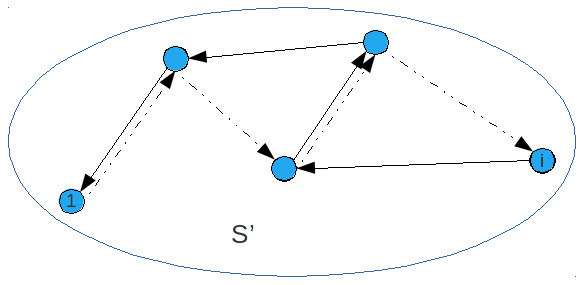
\includegraphics[height=5cm]{images/graph49.png} & 
		Matrice $[c_{ij}]$ asimmetrica
		\begin{equation*}
			\rightarrow\textnormal{ cammino }f'(S,i)
		\end{equation*}
		\begin{equation*}
			\dashrightarrow\textnormal{ cammino }f(S,i)
		\end{equation*}
	\end{tabular}
\end{table}
Se $c[c_{ij}]$ è simmetrica allora $f'(S,i)=f(S,i)$.\\
Per calcolare $f'(S,i)$ si può usare la stessa ricorsione utilizzata per calcolare $f(S,i)$ ma usando la trasposta della matrice $[c_{ij}]$.\\
In modo simile si possono calcolare le funzioni $f'(k,1)$, $f'(q,i)$.

\subsection{Algoritmo DP+Lower Bound per il TSP}
È la combinazione della "ricorsione forward" con la reverse function $f'(k,1)$ per eliminare stati che non possono condurre ad alcuna soluzione ottima.\\
Al posto di $f'(k,i)$ si può usare $f'(q,i)$ o qualsiasi altra funzione che derivi da un diverso rilassamento dello spazio degli stati.

Sia $z^{*}$ il costo del $TSP$ ottimo.

Se lo stato $(S,i)$ fa parte della soluzione ottima di costo $z^{*}$ allora

\begin{table}[!h]
	\begin{tabular}{m{8cm} m{7.5cm}}
		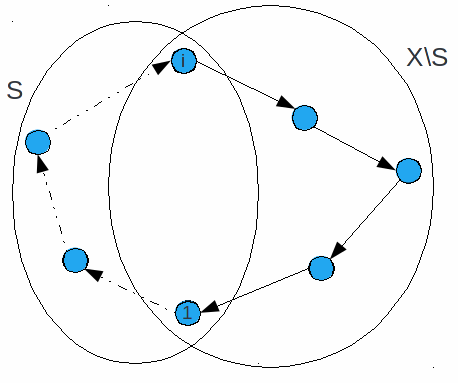
\includegraphics[height=4cm]{images/graph50.png} &
		\begin{equation*}
			f(S,i)+f'(X\setminus S,i)=z^{*}
		\end{equation*}
	\end{tabular}
\end{table}
Sia $z_{UB}$ un upper bound a $z^{*}$ calcolato con un euristico. Sia $k=|S|$ per cui $|X\setminus S|=n-k$.

Lo stato $(S,i)$ non può far parte del $TSP$ ottimo se:
\begin{equation*}
	f(S,i)+
	\begin{cases}
		f'(n-k,i),\ \textnormal{se }\pi'(n-k,i)\in S \\
		\phi'(n-k,i)\ \textnormal{se }\pi'(n-k,i)\in S
	\end{cases}
	\ge z_{UB}
\end{equation*}

\subsection{Algoritmo di programmazione dinamica per il TSP}
\begin{enumerate}
	\item Poni $\mathscr{L}_{i}\{(\{i\}),1\}$, $f(\{i\},i)=0$, $p(\{i\},i)=1$ e $\mathscr{L}_{r}=\emptyset$, $r=2,\dots,n$. Sia $z_{UB}$ un upper bound al $TSP$. Poni $k=2$;
	\item Espandi ogni stato del set $\mathscr{L}_{k-1}$:\\
	per ogni $(S,i)\in\mathscr{L}_{k-1}$ ripeti lo step 3;
	\item Genera gli stati di $\mathscr{L}_{k}$ raggiungibili da $(S,i)$:\\
	per ogni $j\in\Gamma^{-1}\setminus S$ considera lo stato $(S',j)$ dove $S'=S\cup\{j\}$. Poni $h=f(S,i)+c_{ij}$.\\
	Lo stato $(S',j)$ deve essere "rigettato" nei seguenti casi:
	\begin{itemize}
		\item se $h+f'(n-k,i)\ge z_{UB}$ qualora $\pi'(n-k,i)\notin S'$;
		\item se $h+\phi'(n-k,j)\ge z_{UB}$ qualora $\pi'(n-k,j)\in S'$;
		\item se $(S',j)\in\mathscr{L}_{k}$ e $f(S',j)\le h$.
	\end{itemize}
	Se $(S',j)\notin\mathscr{L}_{k}$ allora poni $\mathscr{L}_{k}=\mathscr{L}_{k}\cup\{(S',j)\}$, $f(S',j)=h$ e $p(S',j)=(S,i)$.\\
	Se $(S',j)in\mathscr{L}_{k}$ e $f(S',j)>h$ allora poni $f(S',j)=h$ e $p(S',j)=(S,i)$;
	\item Poni $k=k+1$; se $k\le n$ vai allo step 2;
	\item L'ottimo è dato da $z^{*}=\underset{(X,j)\in\mathscr{L}_{k}}{Min}[f(X,j)+c_{ji}]$.
\end{enumerate}
